%% LyX 2.3.7 created this file.  For more info, see http://www.lyx.org/.
%% Do not edit unless you really know what you are doing.
\documentclass[12pt]{article}
\usepackage[utf8]{inputenc}
\usepackage[a4paper]{geometry}
\geometry{verbose}
\usepackage{xcolor}
\usepackage{array}
\usepackage{calc}
\usepackage{url}
\usepackage{amsmath}
\usepackage{amsthm}
\usepackage{amssymb}
\usepackage{graphicx}
\usepackage[unicode=true,
 bookmarks=false,
 breaklinks=false,pdfborder={0 0 1},backref=section,colorlinks=false]
 {hyperref}

\makeatletter

%%%%%%%%%%%%%%%%%%%%%%%%%%%%%% LyX specific LaTeX commands.
%% Because html converters don't know tabularnewline
\providecommand{\tabularnewline}{\\}

%%%%%%%%%%%%%%%%%%%%%%%%%%%%%% User specified LaTeX commands.
% Default fixed font does not support bold face
\DeclareFixedFont{\ttb}{T1}{txtt}{bx}{n}{12} % for bold
\DeclareFixedFont{\ttm}{T1}{txtt}{m}{n}{12}  % for normal

% Custom colors
\usepackage{color}
\definecolor{deepblue}{rgb}{0,0,0.5}
\definecolor{deepred}{rgb}{0.6,0,0}
\definecolor{deepgreen}{rgb}{0,0.5,0}

\usepackage{listings}


\newcommand{\exer}[1]{\addtocounter{cptExo}{1}\noindent\fcolorbox{black}{white}{ \large{\textbf{{Exercice \thecptExo} : #1 }}}}

\usepackage{listings}
\usepackage{amsthm}
\newcommand{\prof}{}
% Python style for highlighting
\newcommand{\pythonstyle}{\lstset{
language=Python,
basicstyle=\ttm,
otherkeywords={self},             % Add keywords here
keywordstyle=\ttb\color{deepblue},
emph={MyClass,__init__},          % Custom highlighting
emphstyle=\ttb\color{deepred},    % Custom highlighting style
stringstyle=\color{deepgreen},
frame=tb,                         % Any extra options here
showstringspaces=false,            % 
inputencoding=utf8,
extendedchars=true,
literate={à}{{\`a}}1 {è}{{\`e}}1 {é}{{\'e}}1 {ù}{{\`u}}1 {â}{{\^a}}1 {ô}{{\^o}}1 {û}{{\^u}}1,
}}
\usepackage{multicol}
\newcounter{cptExo}
\setcounter{cptExo}{0}
\usepackage{url}
% Python environment
\lstnewenvironment{python}[1][]
{
\pythonstyle
\lstset{#1}
}
{}

% Python for external files
\newcommand{\pythonexternal}[2][]{{
\pythonstyle
\lstinputlisting[#1]{#2}}}

% Python for inline
\newcommand{\pythoninline}[1]{{\pythonstyle\lstinline!#1!}}



\makeatother

\begin{document}

\newcommand{\numTD}{TD1}
\newcommand{\themeTD}{Analyse en caractères}
\newcommand{\file}{toto.tex}


\begin{center}
\begin{tabular}{|p{2cm}p{14cm}|}
\hline
{
\includegraphics[width=1.8cm,viewport=0 0 337 248]{../CM/images/sorbonne.png}} & \raisebox{2ex}{\begin{Large}\textbf{Programmation de Modèles Linguistiques (I)}\end{Large}}\\

%2019-2020& \raisebox{2ex}{\begin{large}\textbf{L5SOPROG L3 Sciences du Langage}\end{large}}\\
2023-2024& \raisebox{2ex}{(L5SOPROG L3 Sciences du Langage)}\\
   & \begin{large}\textbf{\numTD}\end{large} \begin{large} \textbf{\themeTD}\end{large} \\
&\\
& Caroline Koudoro-Parfait et Gaël Lejeune, Sorbonne Université \\
\hline
\end{tabular}
\end{center}


\hrule
%%%%%%%%%%%%%%%%%%%%%%%%%EN-TETE%%%%%%%%%%%%%%%%%%%%%%%%%%%%%
%\renewcommand{\contentsname}{Sommaire du TD}
%\tableofcontents
%\newpage

\noindent\fcolorbox{red}{lightgray}{
\begin{minipage}{12cm}
\section*{Objectifs}

\begin{itemize}
 \item Faire des manipulations simples sur un texte 
 \item Identifier les propriétés morphologiques d'une langue
 \item Les comparer à d'autres
\end{itemize}
\end{minipage}
}
\newline

\exer{Distribution des mots selon la taille en caractères}


 Nous allons implanter le calcul de la distribution des mots d'un texte (son vocabulaire) en fonction de leur taille en caractères.
 Ainsi, vous devrez calculer le nombre de mots uniques pour une taille donnée comme le montre la Figure \ref{distrib}.

\begin{figure}[h]
  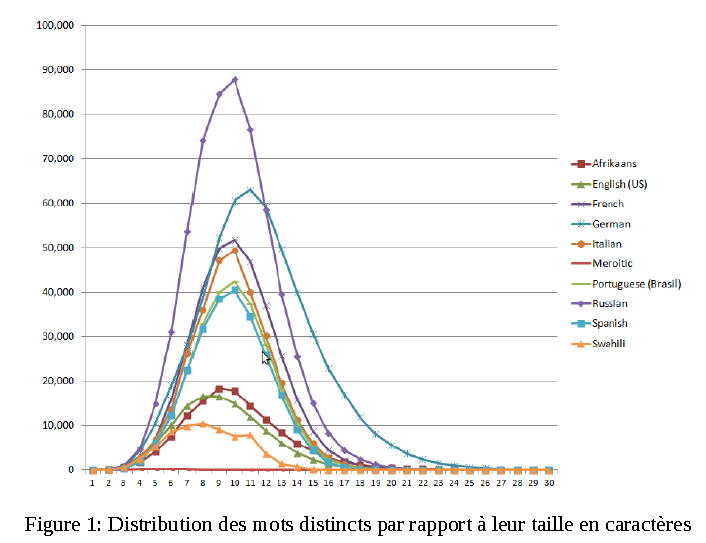
\includegraphics[trim = {0cm 1.5cm 0cm 0cm}, clip, width=.6\textwidth]{images/distrib.png}
  \caption{Distribution des mots par rapport à leur taille en caractères dans différentes langues\label{distrib}}
\end{figure}


 L'axe des abscisses représente la taille d'un mot en caractères et l'axe des ordonnées représente le nombre de mots uniques correspondant à cette taille.

Pour préparer votre espace de travail sur votre notebook  \textsc{Jupyter}, créez un dossier TD1 dans lequel vous enregistrerez votre code et vos données.

 Pous constituer un corpus, vous utiliserez les fichiers textes suivants (choisissez plain text utf-8):
\begin{itemize}
\item "Le discours de la méthode" (fr) \url{http://www.gutenberg.org/ebooks/13846} %. Pour que les résultats soient plus significatifs, pensez à supprimer les premières phrases du fichier écrites en anglais.
\item "Ulysses" (en) \url{http://www.gutenberg.org/ebooks/4300}
\end{itemize}

\newpage

\textbf{Les étapes :}

\begin{enumerate}
  \item  \textbf{lire} les textes
  \item  \textbf{découper} en mots (ou tokeniser)
  \item  \textbf{compter} le nombre de mots par taille de caractères
  \item  \textbf{observer} les résultats chiffrés
  \item  \textbf{représenter} cela sur une courbe
\end{enumerate}


\textbf{Etape 1 : lire}

On ouvre le fichier en indiquant son chemin (\textit{path}), si vous avez bien enregistré votre fichier au même endroit que votre code, le nom du fichier suffit
.

\textbf{Si ça ne marche pas c'est que} :
\begin{itemize}
  \item Tout n'est pas au bon endroit (\texttt{File not Found}), regardez dans l'onglet \texttt{files} de \textsc{Jupyter} pour voir où vous êtes.
  \item ou que on a un problème d'encoding (\texttt{charmap}), il faut ajouter ecoding ='utf-8' dans le open : open("13846-0.txt", encoding ="utf-8")
\end{itemize}

Nous allons commencer par le "Discours de la Méthode", si vous avez conservé le nom d'origine il devrait s'appeler "13846-0.txt".

\begin{python}
with open("13846-0.txt") as f:
  chaine = f.read()
\end{python}

Et on affiche un bout du texte pour vérifier que ça marche :

\begin{python}
print(chaine[:100])
\end{python}


\textbf{Etape 2 : découper}

On va très simplement découper en mots avec la \textbf{méthode} \textit{split}
\begin{python}
liste_mots = chaine.split()#approximation des occurrences
print("Nombre de mots : %i" %len(liste_mots))
\end{python}


\textbf{Etape 3 : compter}

On va utiliser un \textbf{dictionnaire} (ou tableau associatif) où l'on va stocker pour chaque longueur en caractères le nombre de mots qu'on a rencontré. Le fonctionnement est le suivant:
\begin{itemize}
  \item pour chaque mot de la liste de mots, on calcule sa longueur
  \item on vérifie si on a déjà rencontré un mot de cette longueur:
  \begin{itemize}
    \item Si c'est le premier mot pour cette longueur on crée une \textbf{clé} pour cette longueur à laquelle on affecte la \textbf{valeur} 1
    \item Sinon, on \textbf{incrémente} de 1 la valeur existante
  \end{itemize}
\end{itemize}

\begin{python}
dic_longueurs = {} #un dictionnaire vide

for mot in liste_mots:
  longueur = len(mot)#la longueur du mot
  if longueur not in dic_longueurs: #on a jamais vu cette longueur de mot
    dic_longueurs[longueur]=1 #
  else: #on a vu cette longueur de mot
    dic_longueurs[longueur]+=1

print(dic_longueurs)#pour avoir une vue de ce qu'on a fait

\end{python}

NB: si le processus ne vous semble pas clair, ajoutez au début de la boucle \textit{for} deux lignes (avec l'indentation) pour suivre le processus pas à pas :

\begin{python}
  print(dic_longueurs)
  dd=input("Appuyez sur Enter pour passer a la suite")
\end{python}

\textbf{Etape 4: observer}

Un dictionnaire n'est pas une structure de données ordonnée, pour vérifier que'on trouve des résultats proche de l'attendu, on va afficher le nombre d'occurences enregistré dans \texttt{dic\_longueurs} pour toutes les longueurs de 1 à 30 en utilisant \textbf{l'itérateur} \textit{range}. Dans le \textit{print} on utilise du \textbf{formatage de chaînes de caractères}\footnote{Voir par exemple \url{https://stackoverflow.com/questions/5082452/string-formatting-vs-format}}.

\begin{python}
for toto in range(1, 31):#de 1 à 30 (31 est exclu)
  nbr_occurences = dic_longueurs[toto]
  print("%i : %i"%(toto, nbr_occurences))
\end{python}

Vous verrez que le code plante car on a des longueurs qui ne sont pas dans le dictionnaire, on va donc améliorer le code de la façon suivante:

\begin{python}
for toto in range(30):
  if toto in dic_longueurs:
    nbr_occurences = dic_longueurs[toto]
    print("%i : %i"%(toto, nbr_occurences))
  else:
    nbr_occurences = 0 
    print("%i : %i"%(toto, nbr_occurences))
\end{python}


\textbf{Etape 5 : représenter}

Et maintenant c'est magique, on va créer une courbe grâce à la librairie \texttt{matplotlib}. On va importer cette librairie et la renommer pour que ça soit plus court à écrire. Puis pour avoir les valeurs à mettre sur la courbe on va lire les valeurs dans l'ordre croissant pour les ranger dans une liste nommée \textit{liste\_effectifs}. Pyplot prend entrée un \textbf{vecteur}, une liste de valeurs ordonnées.

\begin{python}
import matplotlib.pyplot as pyplot #import avec alias

liste_effectifs = []
for toto in range(30):
  if toto in dic_longueurs:#on a donc vu des mots de cette longueur
    liste_effectifs.append(dic_longueurs[toto])
  else:#on en n'a pas vu de cette longueur, on ajoute donc un 0
    liste_effectifs.append(0)
pyplot.plot(liste_effectifs)#on "dessine"
pyplot.show()#"on affiche"

\end{python}

\begin{figure}
\begin{center}
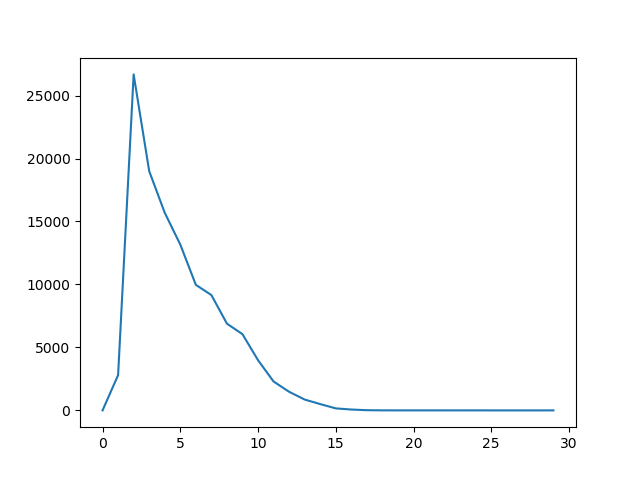
\includegraphics[width=.5\textwidth]{images/TD1_effectifs1.png}
\caption{"Discours de la Méthode" : nombre de mots par longueur (en abscisse), en ordonnée l'effectif}
\end{center}
\end{figure}


Maintenant si on veut faire le même calcul pour l'autre texte on a juste à changer le nom du fichier dans l'étape 1 et à relancer toutes les cellules. Mais si on avait 100 textes à faire ça ne serait pas très pratique. Nous allons donc voir dans l'exercice suivant comment améliorer le code.


\newpage
\exer{Factorisation du code}

 Pour améliorer nous allons construire des \textbf{fonctions} pour \textbf{factoriser} les traitements et constituer une \textbf{chaîne de traitement} fiable.

\textbf{Etape 1: lire}

Ce qui va changer ici c'est qu'on veut traiter plusieurs textes facilement. Bien sûr on pourrait faire :

\begin{python}
with open("13846-0.txt") as f:#Discours de la Methode
  chaine1 = f.read()
with open("4300-0.txt") as f:#Ulysses
  chaine2 = f.read()
\end{python}
 La première chose que l'on remarque c'est que sur Windows (le problème ne se pose pas avec Mac ou Linux) on arrive à ouvrir le texte en anglais mais pas celui en français. C'est un problème d'encodage des caractères (\texttt{charmap} error). L'encodage c'est la manière dont on stocke les caractères en les changeant en "0" et en "1".
 Pour faire simple, quand on a des caractères accentués on a besoin d'un encodage (\textit{encoding}) adapté. Ici c'est "utf-8", on va faire la modification suivante :
\begin{python}
with open("13846-0.txt", encoding='utf-8') as f:#Discours de la Methode
  chaine1 = f.read()

with open("4300-0.txt") as f:#Ulysses
  chaine2 = f.read()
\end{python}

 On voit que l'on a répété deux fois le même code et aussi que si l'on a des correctiosn à faire, il faudra le faire deux fois.

 Si on a 100 textes à traiter il faut 300 lignes de code, pas très pratique.Nous allons voir avec une fonction ça marche mieux. Pour la fabriquer il faut décomposer notre problème, voir \textbf{ce qui est constant} (factorisable, les opérations) et \textbf{ce qui est variable} (non factorisable, paramètre ou sortie de la fonction).
 On se rend vite compte que ce que l'on veut c'est à partir d'un chemin de fichier (\textbf{input} ou entrant) avoir son contenu sous forme de chaîne de caractères (\textbf{output} ou sortant). Ce qui nous donne :

\begin{python}
def lire_fichier(chemin):
  with open(chemin, encoding = 'utf-8') as f:
    chaine = f.read()
  return chaine

chaine1 = lire_fichier("13846-0.txt")#Discours de la Methode
chaine2 = lire_fichier("4300-0.txt")#Ulysses

\end{python}

\textbf{Etape 2 : découper}

Toujours réfléchir en terme d'entrant/sortant : Quel est l'entrant et le  sortant qu'il faut ajouter dans le squelette ci-contre à la place des XXX, YYY et ZZZ?

\begin{python}
def decouper_en_mots(XXX):
  #on decoupe
  liste_mots = YYY
  return ZZZ

\end{python}

(à vous de réfléchir, réponse page suivante)
\newpage

\begin{python}
def decouper_en_mots(chaine):
  #on decoupe
  liste_mots = chaine.split()
  return liste_mots

liste_mots1 = decouper_en_mots(chaine1)
liste_mots2 = decouper_en_mots(chaine2)
\end{python}

\textbf{Etape 3 : compter}
	
En entrée : la liste de mots

En sortie : les effectifs

NB: vous pouvez mettre des \textit{print} quand vous testez pour bien voir ce qu'il se passe.

\begin{python}

def get_effectifs(liste_mots):
  dic_longueurs = {}
  for mot in liste_mots:
    longueur = len(mot)#la longueur du mot
    if longueur not in dic_longueurs: #on a jamais vu cette longueur de mot
      dic_longueurs[longueur]=1 #
    else: #on a vu cette longueur de mot
      dic_longueurs[longueur]+=1
  return dic_longueurs

\end{python}

Et cette fonction on va l'utiliser directement dans l'étape 5

\textbf{Etape 4 : observer (obsolète)}

 C'était une étape de vérification devenue inutile puisqu'on n'a pas changé les opérations effectuées. 

\textbf{Etape 5 : représenter}

Ici on va pouvoir afficher les deux courbes sur la même figure et cerise sur le gâteau on va la sauvegarder.

\begin{python}
import matplotlib.pyplot as pyplot #import avec alias

for liste in [liste_mots1, liste_mots2]: #on a une liste de liste pour factoriser
  dic_longueurs = get_effectifs(liste)
  liste_effectifs = []
  for toto in range(30):
    if toto in dic_longueurs:#on a donc vu des mots de cette longueur
      liste_effectifs.append(dic_longueurs[toto])
    else:#on en n'a pas vu de cette longueur, on ajoute donc un 0
      liste_effectifs.append(0)
  pyplot.plot(liste_effectifs)#on "dessine" mais dans la boucle

pyplot.show()#"on affiche" mais hors de la boucle (pour avoir tout)

\end{python}

\begin{figure}
\begin{center}
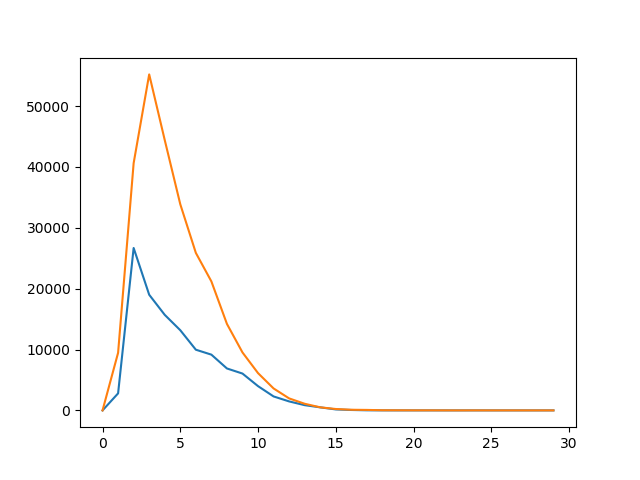
\includegraphics[width=.5\textwidth]{images/TD1_effectifs_total.png}
\caption{"Discours de la Méthode" et "Ulysses" : nombre de mots par longueur (en abscisse), en ordonnée l'effectif}
\end{center}
\end{figure}

On se rend compte que la figure est difficile à interpréter, en effet on travaille en valeur absolue alors que les textes sont de taille différente. On va donc utiliser la taille de chaque texte en mots (avec la fonction \texttt{len}) pour  avoir cette fois une figure avec la proportion de mots de chaque longueur :

\newpage

\begin{python}
#On remplace la ligne :
      liste_effectifs.append(dic_longueurs[toto])
#Par:
      liste_effectifs.append(dic_longueurs[toto]/len(liste))
\end{python}

\begin{figure}
\begin{center}
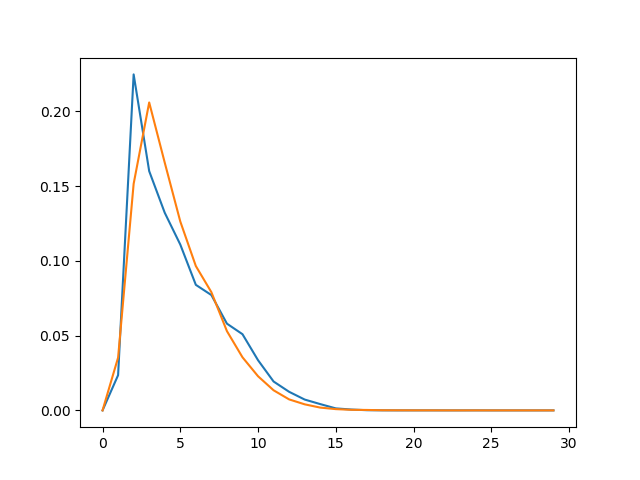
\includegraphics[width=.5\textwidth]{images/TD1_frequences_total.png}
\caption{"Discours de la Méthode" et "Ulysses" : nombre de mots par longueur (en abscisse), en ordonnée la fréquence}
\end{center}
\end{figure}

Voir page suivante pour un bilan

\newpage
\textbf{Après une dernière étape de factorisation voici où nous en sommes :}

\begin{python}
def lire_fichier(chemin):
  with open(chemin, encoding = "utf-8") as f:
    chaine = f.read()
  return chaine

def decouper_en_mots(chaine):
  liste_mots = chaine.split()
  return liste_mots

def get_effectifs(liste_mots):
  dic_longueurs = {}
  for mot in liste_mots:
    longueur = len(mot)
    if longueur not in dic_longueurs:
      dic_longueurs[longueur]=1 
    else:
      dic_longueurs[longueur]+=1
  return dic_longueurs

def vecteur_longueurs(dic_longueurs, liste_mots):
  liste_effectifs = []
  for toto in range(30):
    if toto in dic_longueurs:
      liste_effectifs.append(dic_longueurs[toto]/len(liste_mots))
    else:
      liste_effectifs.append(0)
  return liste_effectifs

import matplotlib.pyplot as pyplot

for chemin in ["13846-0.txt", "4300-0.txt"]:
  chaine = lire_fichier(chemin)
  liste_mots = decouper_en_mots(chaine)
  dic_longueurs = get_effectifs(liste_mots)
  liste_effectifs = vecteur_longueurs(dic_longueurs, liste_mots)
  pyplot.plot(liste_effectifs)

pyplot.savefig("frequences.png")#le bonus: on sauvegarde
pyplot.show()


\end{python}

C'est pas mal, au prochain TD on améliorera le rendu de la figure (légende, échelle) et on travaillera sur plus de langues.


%\exer{Bonus : améliorations}
%%\begin{python}
%%print("texte")
%%\end{python}


\end{document}
